\documentclass[a4paper]{report}
\usepackage[T1]{fontenc}%per rappresentare i font italiani, come le lettere accentate, con la giusta spaziatura
\usepackage[utf8]{inputenc}%per poter inserire nel testo .tex i caratteri unicode8
\usepackage[italian]{babel}%per poter effettuare la giusta sillabazione della lingua italiana
\usepackage{amsmath}%per poter rappresentare ed utilizzare al meglio gli ambienti e le formule matematiche
\usepackage{amssymb}%per rappresentare alcuni simboli particolari matematici
\usepackage{amsthm}
%\usepackage{amsfont}%per poter avere i font matematici
\usepackage{booktabs}
\usepackage{graphics}
\usepackage{pgfplots}
\usepackage{rotating}
\usepackage{microtype}%per effettuare un aggiustamento della spaziatura tra caratteri e del font
\usepackage{url}%per poter rappresentare gli url nel testo latex
%\usepackage{hypertext}%per effettuare un collegamento con una pagina internet
\newtheorem{defi}{Definizione}%Definizione per avere la gestione delle definizioni
\newtheorem{prop}{Proposizione}[chapter]
\newtheorem{lem}{Lemma}
\newtheorem{teorema}{Teorema}[chapter]
\newtheorem{corol}{Corollario}[chapter]


\begin{document}
%Intestazione e indice dei contenuti
\title{Linguaggi di Programmazione}
\author{Marco Natali}
\date{}%rappresenta la data di compilazione del file
\maketitle

\tableofcontents

\chapter{Introduzione ai Paradigmi di Programmazione}
Nel corso di Linguaggi di Programmazione ci occupiamo di 3 importanti paradigmi di 
di linguaggi quali i linguaggi logici, linguaggi funzionali e linguaggi predicativi.

Durante il corso, e soprattutto durante la vita futura lavorativa, si devono rispettare le regole
standard di formattazione dei programmi come le regole google, regole gnu ed ecc... ossia nei programmi
devono essere rispettate le seguenti regole:
\begin{itemize}
\item usare Emacs come editor in quanto indenta lui al meglio
\item le linee di codice non devono essere più lunghe di 80 colonne
\item inserire spazi tra gli operatori e uno spazio dopo , e ; ossia 2 + 3 e (4, 5)
\item non inserire uno spazio tra il nome di una funzione/predicato e le parentesi ossia foo(4)
\item inserire uno spazio tra un istruzione di controllo e logica  e le parentesi ossia if (4 || 5)
\item non usare i commenti all'interno di un box perchè difficilmente mantenibile
\end{itemize}
I linguaggi di programmazione vengono classificati in base a dei paradigmi, ossia un modello di riferimento
su come strutturare un programma, al fine di facilitare l'apprendimento di linguaggi similari:
\begin{itemize}
\item Imperative Languages: linguaggi basati sull'architettura di Von Neumann, base di tutti i calcolatori moderni,
      in cui il processore ha il compito di leggere e scrivere le celle di memoria durante l'esecuzione della computazione.\newline
      Questa tipologia di linguaggi utilizza uno stile prescrittivo, ossia i programmi iterativi specificano una sequenza
      di istruzioni da eseguire per modificare lo stato del sistema e questo flusso può essere modificato soltanto con
      le strutture di controllo.
      Fanno parte di questo paradigma il C/C++, i linguaggi Assembler, Pascal, Python, ...
\item Logic Languages: linguaggi in cui un programma è una deduzione logica ossia ogni istruzione è una formula del linguaggio
      e noi interroghiamo il sistema per sapere se una formula del linguaggio fa parte della conoscenza rappresentata nel programma;
      questo paradigma viene utilizzato per la dimostrazione della correttezza di un programma, per rappresentare i database
      ed infine sta avendo un notevole utilizzo ultimamente nel campo dell'AI(Artificial Intelligence).
      Fa parte di questo paradigma principalmente solo il Prolog e i suoi derivati.
\item Functional Languages: linguaggi in cui il concetto di funzione è l'unica cosa importante per cui i programmi definiscono
      funzioni e l'esecuzione consiste nell'applicazione di uno o più funzioni agli argomenti.
      Fanno parte di codesto paradigma i linguaggi Lisp, Common Lisp, Scheme, Javascript, ML, Ocaml, Haskell, R, ...
\end{itemize}
Ogni dei seguenti paradigmi può avere la presenza di linguaggi object oriented, come Java, C++, Comon Lisp, Python, ...,
infatti il paradigma ad oggetti è ortogonale alla definizione dei seguenti paradigmi, anche se presume alcune features tipiche
dei linguaggi imperativi.

\section{Paradigma Imperativo}
Il paradigma imperativo, come già visto durante la definizione dei diversi paradigmi, si occupa di eseguire una sequenza di istruzioni
per effettuare la computazione infatti il paradigma imperativo è stato inventato più per la computazione ``numerica'' rispetto agli
altri paradigmi.

La struttura del programma è composta da due componenti, una per rappresentare le strutture dati e l'altra per gli algoritmi:
\begin{itemize}
\item dichiarazione: istruzioni in cui vengono dichiarate le variabili, i tipi e le funzioni necessarie per effettuare
  la computazione, ossia vengono definite le strutture dati necessarie per eseguire la computazione voluta.
\item definizione: istruzioni in cui vengono implementati gli algoritmi, per eseguire correttamente la computazione, attraverso
  l'utilizzo di istruzione facenti parte del linguaggio.
\end{itemize}

%Inserire esempio di Programma Imperativo

\section{Paradigma Logico}
La necessità di gestire le applicazione ad un maggiore livello di astrazione e di scrivere programmi il più concisi possibile ha spinto
alla creazione di nuovi paradigmi, come quello logico che analizzeremo ora.

Il paradigma logico non è più basato sull'architettura di Von Neumann ma su concetti matematici, come la logica matematica,
ed utilizza uno stile di programmazione descrittivo, ossia viene definito cosa fa parte e cosa no del problema da rappresentare.

Inoltre nella programmazione logica non è presente alcuna separazione netta tra gli algoritmi e le strutture dati e, come già
visto nella separazione tra i vari paradigmi, un programma consiste nel descrivere un problema come una serie di sentenze del linguaggio
ed interrogare il sistema, il quale effettua una deduzione sulla base della conoscenza rappresentata.

Un esempio di programma logico è il seguente:
%Inserisci file employees.pl


\section{Paradigma Funzionale}
Il paradigma funzionale, come visto nel paradigma logico, viene usato per una programmazione simbolica, è basata su concetti matematici,
adotta solitamente uno stile descrittivo di programmazione ed infine non vi è una completa separazione tra strutture dati ed algoritmi.

Il concetto fondamentale di questo paradigma è la funzione, che è una relazione tra due insiemi che associa un elemento del dominio uno e
un solo elemento del codominio.

Dopo che è stata definita una funzione, possiamo applicarla su un elemento del dominio per ottenere un valutazione della funzione per cui
un programma funzionale si riduce alla valutazione di una funzione per ottenere un valore, in cui in un linguaggio funzionale puro esso è
determinato soltanto dalla funzione e non da i valori in memoria.\newline
Questa assenza di effetti dati dalla memoria consiste nel definire una variabile come una costante matematica ossia il valore non è mutabile
a differenza delle variabili nei linguaggi imperativi che sono una astrazione di una locazione in memoria.

Un programma funzionale, come già visto nella definizione dei vari paradigmi, consiste nella definizione di un insieme di funzioni,
eventualmente ricorsive, e l'esecuzione di un programma consiste nell'applicazione di una funzione agli argomenti.

Esempio di programma funzionale:

\section{Richiami sugli ambienti RunTime e architettura degli elaboratori}
Per eseguire un programma in un qualsiasi linguaggio il sistema (ovvero il sistema operativo) deve mettere a disposizione
un ambiente \textit{run time}, che può essere anche una macchina virtuale, il quale fornisce almeno due funzionalità:
\begin{itemize}
\item mantenimento dello stato della computazione (program counter, limiti di memoria etc)
\item gestione della memoria disponibile (fisica e virtuale)
\end{itemize}

La gestione della memoria avviene usando due aree concettualmente ben distinte con funzioni diverse:
\begin{itemize}
\item lo \textit{Stack}  serve per la gestione delle chiamate (soprattutto ricorsive) a procedure, metodi, funzioni etc...(record di attivazione).
\item lo \textit{Heap} serve per la gestione di strutture dati dinamiche (liste, alberi etc...)
\end{itemize}
I linguaggi logici e funzionali (ma anche Java) utilizzano pesantemente lo Heap dato che forniscono come strutture dati built-in 
liste e spesso vettori di dimensione variabile.

La gestione dei record di attivazione è stata affrontata nei corsi di Programmazione ed Architettura, a cui si può consultare i
libri e gli appunti per rinfrescare la memoria.

La gestione della memoria, in particolare quella dinamica, può avvenire in maniera automatica, attraverso il \emph{Garbage Collector} che è
usato da Python, Java, Lisp, Prolog ed altri, oppure in maniera manuale, come in C/C++ attraverso i comandi malloc(new) e free(delete).

\chapter{Ripasso Logica Proposizionale e Predicativa}
Effettuiamo ora un ripasso della logica proposizionale e predicativa, affrontata nel corso Fondamenti dell'Informatica, al fine di rivedere
e perfezionare i concetti di logica necessari per la comprensione e la scrittura di programmi logici.

Partiamo con l'esempio di una semplice dimostrazione geometrica effettuata con le regole della logica:
\begin{teorema}
  Dato un triangolo isoscele (con $\overline{AB}=\overline{BC}$) si ha che $\angle A$, ovvero l'angolo in $A$,
  e $\angle C$, ovvero l'angolo in $C$, sono uguali.
\begin{center}
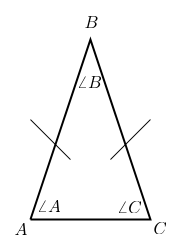
\includegraphics[scale=0.5]{img/tri.png}
\end{center}
\end{teorema}
\begin{proof}
Si comincia la dimostrazione con l'elenco delle conoscenze pregresse: 
\begin{enumerate}
\item se due triangoli sono uguali essi hanno lati e angoli uguali
\item se due triangoli hanno due lati e l'angolo sotteso uguale allora i due triangoli sono uguali
\item se viene definita la bisettrice di $\angle B$, $\overline{BH}$, si ha che $\angle ABH = \angle HBC$
\begin{center}
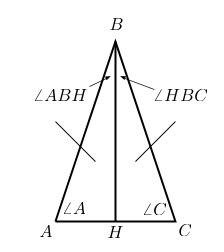
\includegraphics[scale=0.5]{img/tri2.png}
\end{center}
\end{enumerate}
Procediamo ora coi passi della dimostrazione:
\begin{enumerate}
\item $\overline{AB}=\overline{BC}$ per ipotesi
\item $\angle ABH = \angle HBC$ per la terza conoscenza pregressa
\item $\triangle HBC = \triangle ABH$ per la seconda conoscenza pregressa in quanto due lati sono uguali per ipotesi e dal passo precedente
      l'angolo sotteso ai due lati uguali è uguale in ambedue i triangoli.
\item $\angle A= \angle C$ per la prima conoscenza pregressa dato che $\triangle HBC = \triangle ABH$ 
\end{enumerate}
Siamo così giunti alla fine della dimostrazione ma adesso vogliamo rappresentarla attraverso gli strumenti della logica al fine di rendere
totalmente formale la dimostrazione per cui si effettua i seguenti passaggi:
\begin{itemize}
\item si è trasformata la seconda conoscenza pregressa in:\newline
  \textbf{se} $\overline{AB}=\overline{BC}$ \textbf{e} $\overline{BH}=\overline{BH}$ \textbf{e} $\angle ABH = \angle HBC$
  \textbf{allora} $\triangle ABH=\triangle HBC$
\item si è trasformata la prima conoscenza pregressa in:\newline
  \textbf{se} $\triangle ABH=\triangle HBC$ \textbf{allora} $\overline{AB}=\overline{BC}$ \textbf{e} $\overline{BH}=\overline{BH}$
  \textbf{e} $\overline{AH}=\overline{HC}$ \textbf{e} $\angle ABH = \angle HBC$ \textbf{e} $\angle AHB = \angle CBH$ \textbf{e} $\angle A=\angle C$
\end{itemize}
Possiamo ora procedere col processo di formalizzazione, ossia il processo che ci permette di affermare
$\overline{AB} = \overline{BC} \vdash \angle A = \angle C$ con $\vdash$ simbolo di derivazione logica, che significa consegue, allora, ecc...

Assumendo $P = \{ \overline{AB} = \overline{BC}, \angle ABH = \angle HBC, \overline{BH} = \overline{BH} \}$
ed avendo le seguenti conoscenze pregresse:
\begin{enumerate}
\item $\overline{AB}=\overline{BC} \land \overline{BH}=\overline{BH} \land \angle ABH = \angle HBC \rightarrow \triangle ABH=\triangle HBC$
\item  $\triangle ABH=\triangle HBC \rightarrow \overline{AB}=\overline{BC} \land \overline{BH}=\overline{BH} \land \overline{AH}=\overline{HC}
        \land \angle ABH = \angle HBC \land \angle AHB = \angle CBH \land \angle A=\angle C.
\end{enumerate}
per ottenere $\overline{AB} = \overline{BC} \vdash \angle A = \angle C$ bisogna effettuare la seguente catena:
\begin{enumerate}
\item \textbf{P1:} $\overline{AB}=\overline{BC}$ preso da \textbf{P}
\item \textbf{P2:} $\angle ABH = \angle HBC$ preso da \textbf{P}
\item \textbf{P3:} $\overline{BH}=\overline{BH}$ preso da \textbf{P}
\item \textbf{P4:} $\overline{AB} = \overline{BC} \land \overline{BH} = \overline{BH} \land \angle ABH = \angle HBC$ preso da \textbf{P1, P2, P3} e       dalla regola \textbf{introduzione della congiunzione}.
\item \textbf{P5:} $\triangle ABH = \triangle HBC$ da \textbf{P4}, dalla \textbf{regola 2}  e dalla regola di inferenza detta \textbf{modus ponens}.
\item \textbf{P6:} $\overline{AB} = \overline{BC} \land \overline{BH} = \overline{BH} \land \overline{AH} = \overline{HC} \land
  \angle ABH = \angle HBC \land \angle AHB = \angle CBH \land \angle A=\angle C$ da \textbf{P5}, dalla \textbf{regola 1} e dalla regola
  \textbf{modus ponens}.
\item \textbf{P7:} $\angle A=\angle C$ da \textbf{P6} e dalla regola d'inferenza eliminazione della congiunzione 
\end{enumerate}
Abbiamo così dimostrato tutto anche per mezzo dei costrutti della logica
\end{proof}
\begin{definizione}
Una dimostrazione del tipo \textit{F è conseguenza di S}, \textbf{dim}, si indica con:
$$S\,\,\vdash\,\, F$$
ed è una sequenza:
$$dim=<P_1,P_2,...,P_n>$$
con:
\begin{itemize}
\item $P_n=F$
\item $P_i \in S$ o con $P_i$ ottenibile dalle $P_1,...,P_{i-1}$ applicando una regola di inferenza
\end{itemize}
\end{definizione}
Un insieme di regole di inferenza costituisce la base di un calcolo logico, il quale ha lo scopo di manipolare le formule in modo
unicamente sintattico al fine di stabilire una connessione tra un insieme di formule di partenza, dette assiemi e un insieme di conclusioni.

\subsection{Logica Proporzionale}
La logica proposizionale si occupa delle conclusioni che si possono trarre da un insieme di proposizioni, che definiscono sintatticamente la logica
proposizionale, ma purtroppo è un linguaggio limitato che non si può generalizzare le proposizioni.

La sintassi di un linguaggio è composta da una serie di formule ben formate($FBF$) definite induttivamente nel seguente modo:
%definizione formule ben formate
\begin{enumerate}
  \item Le costanti e le variabili proposizionali $\in FBF$(chiamate atomi o letterali).
  \item Se $A$ e $B \in FBF$ allora $(A \land B)$,$(A \lor B)$,$(\neg A)$,$(A \rightarrow B)$,
        $(A \iff B)$,$TA$ e $FA$ sono delle formule ben formate.
  \item nient'altro è una formula
\end{enumerate}

Esempio:\newline
$(P \land Q) \in Fbf$  è una formula ben formata\newline
$(PQ \land R) \not \in Fbf$ in quanto non si rispetta la sintassi del linguaggio definita.\newline

La semantica di una logica consente di dare un significato e un interpretazione alle formule del Linguaggio.\newline
\begin{defi}
  Sia data una formula proposizionale $P$ e sia ${P_1,\dots,P_n}$, l'insieme degli atomi che compaiono nella formula $A$.
  Si definisce come \emph{interpretazione} una funzione $v:\{P_1,\dots,P_n\} \mapsto \{T,F\}$ che attribuisce un valore di verità
  a ciascun atomo della formula $A$.
\end{defi}
I connettivi della Logica Proposizionale hanno i seguenti valori di verità:
%Tabella di Verità degli operatori
$\begin{array}{ccccccc}
\toprule
\text{A} & \text{B} & A \land B & A \lor B & \neg A & A \Rightarrow B & A \iff B \\
\midrule
    F & F & F & F & T & T & T \\
    F & T & F & T & T & T & F \\
    T & F & F & T & F & F & F \\
    T & T & T & T & F & T & T \\
\bottomrule
\end{array}$\newline

La tavola di verità costituisce la semantica di un insieme di proposizioni mentre un calcolo logico dice come generare nuove formule logiche,
ovvero espressioni sintattiche, a partire dagli assiomi e questo processo di generazione si chiama dimostrazione.

Per ottenere nuove formule dagli assiomi si usa il calcolo proposizionale, che si base su regole di inferenza, ossia regole attraverso
i quali si può derivare una nuova formula ben formata.\newline
Le regole di inferenza analizzate sono le seguenti:
\begin{esempio}[Modus Ponens]
$$\frac{a\to b,\,\,a}{b}$$
\end{esempio}

\begin{esempio}[Modus Tollens]
$$\frac{a\to b, \neg b}{\neg a}$$
\end{esempio}

\begin{esempio}[Eliminazione e Introduzione di $\land$]
$$\frac{P_1\land P_2 \land ... \land P_n}{P_i}\,\,[\mbox{Eliminazione di }\land]$$
\end{esempio}

$$\frac{P_1, P_2,...,P_n}{P_1\land P_2 \land ... \land P_n}\,\,[\mbox{Introduzione di }\land]$$
\end{esempio}
\begin{esempio}[Introduzione di $\lor$]
$$\frac{a}{a \lor b}$$
\end{esempio}

\begin{esempio}
Ecco altre regole utili:
\begin{itemize}
\item \textbf{Terzo Escluso:}
$$\frac{a \lor \neg a}{vero}$$
\item \textbf{Eliminazione di} $\neg$:
$$\frac{\neg \neg a}{a}$$
\item \textbf{Eliminazione di} $\vee$:
$$\frac{a \land vero}{a}$$
\item \textbf{Contraddizione:}
$$\frac{a \lor \neg a}{b}$$
ovvero da una contraddizione posso trarre qualsiasi conseguenza
\end{itemize}
\end{esempio}
Queste regole di inferenza fanno parte del calcolo naturale, detto anche di Gentzen, similare al calcolo tramite Tableaux visto nel corso
di Fondamenti dell'informatica.\newline
Questo tipo di calcolo consiste nel formalizzare i modi di derivare conclusioni a partire dalle premesse, ovvero di derivare direttamente un FBF
mediante una sequenza di passi ben codificati.
La regola del modus ponens  insieme al principio del terzo escluso, posso essere usati anche procedendo per assurdo alla dimostrazione
di una data formula e ciò viene detto \emph{principio di risoluzione}, affrontata poi quando analizziamo il linguaggio Prolog.


Una formula nella logica proposizionale può essere di tre diversi tipi:
%Tipologie di formule
\begin{description}
    \item[valida o tautologica]: la formula è soddisfatta da qualsiasi valutazione della Formula
    \item[Soddisfacibile non Tautologica]:la formula è soddisfatta da qualche valutazione
                        della formula ma non da tutte.
    \item[falsibicabile]:la formula non è soddisfatta da qualche valutazione della formula.
    \item[Contraddizione]:la formula non viene mai soddisfatta
\end{description}

\begin{thm}
$A$ è una formula valida se e solo se $\neg A$ è insoddisfacibile.
$A$ è soddisfacibile se e solo se $\neg A$ è falsibicabile
\end{thm}

Si definisce \emph{modello}, indicato con $M \models A$, tutte le valutazioni booleane
che rendono vera la formula $A$.
Si definisce \emph{contromodello}, indicato con , tutte le valutazioni booleane
che rendono falsa la formula $A$.

La logica proposizionale è decidibile, ossia posso sempre verificare il significato di una formula, infatti esiste
una procedura effettiva che stabilisce la validità o no di una formula, o se questa ad esempio è una tautologia.
In particolare il verificare se una proposizione è tautologica o meno è l’operazione di decibilità principale che si svolge
nel calcolo proposizonale.

\begin{defi}
    Se $M \models A$ per tutti gli $M$, allora $A$ è una tautologia e si indica $\models A$
\end{defi}

\begin{defi}
    Se $M \models A$ per qualche $M$, allora $A$ è soddisfacibile
\end{defi}

\begin{defi}
Se $M \models A$ non è soddisfatta da nessun $M$, allora $A$ è insoddisfacibile
\end{defi}

Una dimostrazione di una formula di una logica può venire tramite:
\begin{itemize}
  \item  \textbf{Metodo diretto}: Data un'ipotesi, attraverso una serie di passi
          si riesce a dimostrare la correttezza della Tesi
  \item \textbf{Metodo per assurdo}(non sempre accettato in tutte le logiche):
        Si nega la tesi ed attraverso una serie di passi si riesce a dimostrare
        la negazione delle ipotesi.
\end{itemize}

\begin{thm}
    Un apparato deduttivo $R$ è completo se, per ogni formula $A \in Fbf$, $\vdash A$
    implica $\models A$
\end{thm}

\begin{thm}
    Un apparato deduttivo $R$ è corretto se, per ogni formula $A \in Fbf$, $\models A$
    implica $\vdash A$
\end{thm}

\subsection{Logica del primo ordine}
La logica del primo ordine, chiamata anche logica predicativa, permette di quantificare i vari fatti ed introduce il concetto di funzione e
predicato per poter esprimere delle proprietà su una serie di individui.

Un linguaggio predicativo $L$ è composto dai seguenti insiemi di simboli:
\begin{enumerate}
    \item insieme di variabili individuali(infiniti) $x,y,z,\dots$
    \item connettivi logici $\land \lor \neg \rightarrow \iff$
    \item quantificatori  $\forall \exists$
    \item simboli ( , )
    \item Costanti proposizionali $T,F$
    \item simbolo di uguaglianza $=$, eventualmente assente
\end{enumerate}
Questa è la parte del linguaggio tipica di ogni linguaggio del primo ordine poi
ogni linguaggio definisce la propria segnatura ossia definisce in maniera autonomo:
\begin{enumerate}
    \item insiemi di simboli di costante $a,b,c,\dots$
    \item simboli di funzione con arieta $f,g,h,\dots$
    \item simboli di predicato $P,Q,Z,\dots$ con arietà
\end{enumerate}

%Esempio
Esempio:Linguaggio della teoria degli insiemi \newline
Costante:$\emptyset$\newline
Predicati:$\in(x,y)$, $=(x,y)$

Esempio:Linguaggio della teoria dei Numeri \newline
Costante:$0$ \newline
Predicati:$<(x,y)$,$=(x,y)$ \newline
Funzioni:$succ(x)$,$+(x,y)$,$*(x,y)$

%Definizione di Termini e Formule ben formate
Per definire le formule ben formate della logica predicativa bisogna prima definire
l'insieme di termini e le formule atomiche.

\begin{defi}
    L'insieme $TERM$ dei termini è definito induttivamente come segue
    \begin{enumerate}
        \item Ogni variabile e costante sono dei Termini
        \item Se $t_1 \dots t_n$ sono dei termini e $f$ è un simbolo di funzione di arietà $n$
              allora $f(t_1,\dots,t_n)$ è un termine
    \end{enumerate}
\end{defi}

\begin{defi}
    L'insieme $ATOM$ delle formule atomiche è definito come:
    \begin{enumerate}
        \item $T$ e $F$ sono degli atomi
        \item Se $t_1$ e $t_2$ sono dei termini, allora $t_1 = t_2$ è un atomo
        \item Se $t_1,\dots,t_n$ sono dei termini e $P$ è un predicato a $n$ argomenti,
              allora $P(t_1,\dots,t_n)$ è un atomo.
    \end{enumerate}
\end{defi}

\begin{defi}
    L'insieme delle formule ben formate($FBF$) di $L$ è definito induttivamente come
    \begin{enumerate}
        \item Ogni atomo è una formula
        \item Se $A,B \in FBF$, allora $\neg A$, $A \land B$,$A \lor B$,$A \rightarrow B$
              e $A \iff B$ appartengono alle formule ben formate
        \item Se $A \in FBF$ e $x$ è una variabile, allora $\forall x A$ e $\exists x A$
              appartengono alle formule ben formate
        \item Nient'altro è una formula
    \end{enumerate}
\end{defi}

%Variabili legate e chiuse
\begin{defi}
    L'insieme $var(t)$ delle variabili di un termine $t$ è definito come segue:
    \begin{itemize}
        \item $var(t) = \{t \}$, se $t$ è una variabile
        \item $var(t) = \emptyset$ se $t$ è una costante
        \item $var(f(t_1,\dots,t_n)) = \bigcup _{i = 1} ^n var(t_i)$
        \item $var(R(t_1,\dots,t_n)) = \bigcup _{i = 1} ^ n var(t_i)$
    \end{itemize}
\end{defi}

%Termini chiusi ed aperti
Si definisce come \emph{aperto} un termine che non contiene variabili altrimenti
si definisce il termine come \emph{chiuso}.\newline
Le variabili nei termini e nelle formule atomiche possono essere libere
in quanto gli unici operatori che "legano" le variabili sono i quantificatori.

Il campo di azione dei quantificatori si riferisce soltanto alla parte in cui
si applica il quantificatore per cui una variabile si dice \emph{libera}
se non ricade nel campo di azione di un quantificatore altrimenti la variabile si dice \emph{vincolata}.

Si aggiunge una nuova regola d'inferenza per la logica dei predicati, l'eliminazione del quantificatore universale $\forall$:
$$\frac{\forall x, T(...,x,...), c\in C}{T(...,c,...)}$$

Abbiamo altre regole di inferenza per il quantificatore esistenziale:
\begin{itemize}
\item Introduzione del quantificatore esistenziale $\exists$:
$$\frac{T(...,c,...), c\in C}{\exists x, T(...,x,...)}$$
\item si hanno le seguente identità:
$$\exists x, \neg T(...,x,...)\equiv \neg\forall x, T)...,x,...)$$
$$\forall x, \neg T(...,x,...)\equiv \neg\exists x, T(...,x,...)$$
\end{itemize}

\chapter{Prolog:Programmazione Logica}
Dopo aver effettuato un ripasso della logica, incominciamo a considerare il Prolog e la programmazione logica:
le basi del PROLOG (PROgramming in LOGic) sono state poste da Robert Kowalski e Marten Van Emdem, mentre la sua progettazione e implementazione,
avvenuta nel 1972 a Marsiglia attraverso Alain Colmerauer e Philippe Roussel.

Si tratta di un linguaggio di programmazione logica basato sulle Clausole di Horn, ovvero un insieme di procedure attivate
da una asserzione iniziale d’obiettivo e la procedura utilizzata da prolog per la computazione è il principio di risoluzione.

Un programma prolog è un formato da un insieme di istruzioni, rappresentanti un sottoinsieme di frasi ben formate della logica del 1° Ordine
e il sistema prolog ha il fine di determinare se una data assunzione è verificata o meno nel programma e sotto quali eventuali vincoli
ciò risulta  verificato.

I componenti basilari di un programma prolog, rappresentanti tutti una clausola di Horn, sono:
\begin{description}
\item [Fatti]: indica una relazione esistente tra due oggetti, che può venire chiama predicato.
               \begin{minted}{Prolog}
                 A.
               \end{minted}
\item [Query]: chiede al sistema se una relazione esiste tra gli oggetti e quindi inizia una deduzione per stabilire se la query
               è una conseguenza diretta del programma, dopo l'applicazione del modus ponens universale per un numero finito di volte.
               \begin{minted}{Prolog}
                 :- B_1, B_2, ..., B_n.
               \end{minted}
 
\item [Regole]: definisce una nuova relazione esistente tra gli oggetti, ossia permette di derivare una nuova conclusione
                da una serie di fatti e regole.
                \begin{minted}{Prolog}
                  A :- B_1, B_2, ..., B_n.
                \end{minted}
\end{description}
I fatti e le regole sono quantificate universalmente mentre una query si intende sempre quantificata esistenzialmente, per cui una query
risponde true se esiste un instanza $\alpha$ che verifica la query altrimenti risponde false.

Le query e le regole le abbiamo definite nella forma generale, ossia possiamo definire regole e query su congiunzioni di termini,
infatti il simbolo ``,'' rappresenta l'operatore logico and, perciò in caso più termini hanno lo stesso simbolo di variabile
l'instanza $\alpha$ deve essere la stessa per stabilire se una query è una conseguenza diretta del programma.

Le regole stabiliscono una relazione di implicazione, indicato con il simbolo :-, infatti definiamo che risulta A se risulta verificato
B_1, B_2, $\dots$, B_n, ovviamente sempre dal punto di vista sintattico.
Per vedere al meglio questo concetto di implicazione vediamo la definizione del concetto di nonno nel linguaggio Prolog:
\begin{minted}{Prolog}
  grandfather(X, Y) :- father(X, Z), father(Z, Y).
\end{minted}
Questa relazione stabilisce che X è il nonno di Y se risulta che esiste un Z tale che X è padre di Z e Z è padre di Y.




\end{document}
